%\documentclass[10pt,preprint,nocopyrightspace,nonatbib]{sigplanconf}
%\documentclass[9pt,preprint]{sig-alternate-no-permission}
%\documentclass[9pt,preprint]{sig-alternate}
%\documentclass[letterpaper,twocolumn,10pt]{article}
%\usepackage{usenix}
%\documentclass[pageno]{jpaper}
%\documentclass[10pt,preprint]{sigplanconf}
\documentclass[sigplan,10pt,anonymous]{acmart}\settopmatter{printfolios=true}
\usepackage{mathptmx} % This is Times font

\setcopyright{none}             %% For review submission
%\conferenceinfo{SOSP'15}{October 4--7, 2015, Monterey, CA}
%\copyrightyear{2015}
% The following \documentclass options may be useful:

% preprint      Remove this option only once the paper is in final form.
% 10pt          To set in 10-point type instead of 9-point.
% 11pt          To set in 11-point type instead of 9-point.
% authoryear    To obtain author/year citation style instead of numeric.

\usepackage{minted}
\usepackage{epsfig}
%\usepackage[utf8x]{inputenc}
\usepackage{algorithm}
\usepackage{amsmath, amssymb}
\usepackage[noend]{algpseudocode}
\usepackage{enumitem}      % adjust spacing in enums
%\usepackage{subfig}
\usepackage{caption}
\usepackage{subcaption}
\usepackage{multirow}
\usepackage{rotating}
\usepackage{wrapfig}
\usepackage{tabu}
\usepackage{pifont}
\usepackage[normalem]{ulem}

\let\bibhang\relax
\let\citename\relax
\let\bibfont\relax
\let\citeauthor\relax
\let\Citeauthor\relax
\let\citefullauthor\relax
\let\citetext\relax
\let\defcitealias\relax
\let\citet\relax
\let\citep\relax
\let\Citep\relax
\let\Citealt\relax
\let\citealt\relax
\let\citealp\relax
\let\Citealp\relax
\let\Citet\relax

\expandafter\let\csname ver@natbib.sty\endcsname\relax

\DeclareCaptionFormat{subfig}{\figurename~#1#2#3}
\DeclareCaptionSubType*{figure}
%\captionsetup[subfigure]{format=subfig,labelsep=colon,labelformat=simple}

\usepackage[natbib=true,backend=bibtex,firstinits=true,style=numeric-comp,sorting=nyt,defernumbers,maxnames=99,maxcitenames=99]{biblatex}
\usepackage{balance}
\usepackage{adjustbox}

\usepackage{pgfplots}
% options for pgfplots
\pgfplotsset{compat=1.8,compat/show suggested version=false}
\usetikzlibrary{plotmarks}
\usetikzlibrary{calc}
%\pgfplotsset{compat=newest}
\pgfplotsset{
   /pgfplots/bar  cycle  list/.style={/pgfplots/cycle  list={%
        {black,fill=black!30!white,mark=none},%
        {black,fill=red!30!white,mark=none},%
        {black,fill=green!30!white,mark=none},%
        {black,fill=yellow!30!white,mark=none},%
        {black,fill=brown!30!white,mark=none},%
     }
   },
}
% begin of externalization
\usetikzlibrary{external}
\tikzexternalize[prefix=out/]
\tikzexternalize
% don't externalize todonotes
%\makeatletter
%\renewcommand{\todo}[2][]{\tikzexternaldisable\@todo[#1]{#2}\tikzexternalenable}
%\makeatother
% end of externalization
\usetikzlibrary{patterns}
\usepgfplotslibrary{groupplots}
\pgfplotsset{
every axis label/.append style={font=\small},
tick label style={font=\small},
}
% options for paragraphs and lists
\setlist{noitemsep,topsep=0pt}
% options for biblatex
\bibliography{refs}
%\renewcommand{\bibfont}{\footnotesize}


\usepackage{fancyhdr}

% Ensure letter paper
\pdfpagewidth=8.5in
\pdfpageheight=11in

%%%%%%%%%%%---SETME-----%%%%%%%%%%%%%
\newcommand{\microsubmissionnumber}{440}
\newcommand{\asplossubmissionnumber}{440}
%%%%%%%%%%%%%%%%%%%%%%%%%%%%%%%%%%%%

\fancypagestyle{firstpage}{
%   \fancyhf{}
% \setlength{\headheight}{50pt}
% \renewcommand{\headrulewidth}{0pt}
%   \fancyhead[C]{\normalsize{CONFIDENTIAL DRAFT --- DO NOT DISTRIBUTE}}
%   \pagenumbering{arabic}
}

\pagenumbering{arabic}


\setlength{\itemsep}{0pt}
%\setlength{\topsep}{0pt}
%\setlength{\partopsep}{0pt}
%\setlength{\parsep}{1pt}
%\setlength{\parskip}{1pt}
\setlength{\abovecaptionskip}{1pt plus 2pt minus 2pt}
\setlength{\textfloatsep}{5pt}
%\setlength{\bibitemsep}{0pt}

\sloppy

\newif{\ifanonymous}
\anonymoustrue

%\newcommand{\comment}[[1]{\textcolor{red}{#1}}
\newcommand{\myworries}[1]{\textcolor{red}{#1}}
\newcommand{\cutout}[1]{}
\newcommand{\smallcaption}[1]{\caption[#1]{{\protect\small \protect\bf #1}}}
\newcommand{\dids}{{\sc dids}}

\graphicspath{{./figs/}}
\date{}

\algnewcommand{\LineComment}[1]{\(\triangleright\) #1}

% some useful shortcuts
\newcommand{\ie}{\textit{i.e., }}
\newcommand{\eg}{\textit{e.g., }}
\newcommand{\CC}{C\nolinebreak\hspace{-.05em}\raisebox{.5ex}{\tiny\bf +}\nolinebreak\hspace{-.10em}\raisebox{.5ex}{\tiny\bf +}}

% units for results
\newcommand{\us}{\,$\mu$s}
\newcommand{\ms}{\,ms}
\newcommand{\KB}{\,KB}
\newcommand{\MB}{\,MB}
\newcommand{\GB}{\,GB}
\newcommand{\MHz}{\,MHz}
\newcommand{\GHz}{\,GHz}

% new latex commands:
%   Remove long section
\newcommand{\PUNT}[1]{}
\newcommand{\TABLETWO}[1]{}
%   Label work to be done
\definecolor{gray}{gray}{0.75}
\newcommand{\TODO}[1]{\textcolor{gray}{\textbf{\ [TODO:\ #1]\ }}}
\newcommand{\TR}[1]{#1}
%\newcommand{\TR}[1]{}
%\newcommand{\TODO}[1]{}
\newcommand{\FIX}[1] {\textcolor{red}{\textbf{\ [FIX:\ #1]\ }}}
%   Referencing various pieces of the document:
\newcommand{\figref}[1]{Fig.~\ref{fig:#1}}
\newcommand{\figsref}[2]{Figures~\ref{fig:#1} and~\ref{fig:#2}}
\newcommand{\figrref}[2]{Figures~\ref{fig:#1}--\ref{fig:#2}}
\newcommand{\secref}[1]{Section~\ref{sec:#1}}
\newcommand{\secsref}[2]{Sections~\ref{sec:#1} and~\ref{sec:#2}}
\newcommand{\eqnref}[1]{Eqn.~\ref{eqn:#1}}
\newcommand{\eqnsref}[2]{Equations~\ref{eqn:#1} and~\ref{eqn:#2}}
\newcommand{\eqnrref}[2]{Equations~\ref{eqn:#1}--\ref{eqn:#2}}
\newcommand{\insref}[1]{Instruction~\ref{ins:#1}}
\newcommand{\tblref}[1]{Table~\ref{tbl:#1}}
\newcommand{\appref}[1]{Appendix~\ref{app:#1}}

\newcommand{\algoref}[1]{Algorithm~\ref{algo:#1}}

% Custom hyphenation rules

%\DeclareMathOperator{\minimize}{minimize}
%\DeclareMathOperator{\st}{s.t.}
%\DeclareMathOperator*{\argmin}{arg\,min}
%\DeclareMathOperator*{\argmax}{arg\,max}
\newcommand{\argmin}{\arg\!\min}
\newcommand{\argmax}{\arg\!\max}
\newcommand{\minimize}{minimize}
\newcommand{\optimize}{optimize}
\newcommand{\ceil}[1]{\lceil #1 \rceil}
\newcommand{\floor}[1]{\lfloor #1 \rfloor}
\newcommand{\st}{s.t.}

\newcommand{\SYSTEM}{DNSCHK}
\newcommand{\CONFERENCE}{Usenix}

\pdfstringdefDisableCommands{
    \def\\{}
    \def\unskip{}
    \def\texttt#1{<#1>}
}

%-------------------------------------------------------------------------
\begin{document}

\date{}
\title[\SYSTEM{}]{\SYSTEM{}: Malicious Download Detection with Highly-Available Distributed Systems}

\author{
% Not used?
}

\begin{abstract}

  Downloading resources over the internet comes with many risks,
  including the chance that a malicious actor has replaced the
  resource you think you are accessing with a compromised version. The
  current standard for addressing this risk is the use of
  \emph{checksums} coupled with a secure transport layer: users
  download a resource and compare its checksum with a posted checksum
  from the developers to ensure a match. Among the many problems with
  the current use of checksums are (1) user apathy---for most users,
  hand-calculating the checksum and comparing to the published version
  are too tedious---and (2) co-hosting resources and checksums---a
  malicious actor who compromises a resource can trivially compromise
  a checksum a hosted using the same infrastructure. In this paper we
  propose \SYSTEM{}, a novel resource validation scheme meant as a
  complete replacement for current checksum based approaches.
  \SYSTEM{} automates the tedious parts of verification to eliminate
  user apathy while leveraging highly-available distributed systems to
  separate resources from digests, making these systems and their end
  users more resilient to resource integrity attacks.  We carefully
  evaluate the security, performance, and practicality of \SYSTEM{}
  through implementing extensions in both a web browser (Chrome) and
  FTP client (FileZilla); implementations are tested versus common
  resource integrity violations. We find that \SYSTEM{} is more
  effective than existing solutions, detects a wide variety of
  real-world integrity errors across a diverse set of platforms, and
  is a scalable and immediately deployable solution.

\end{abstract}


\maketitle
\thispagestyle{firstpage}
\pagestyle{plain}

%\vskip -100pt

%\category{C.1.3}{Other Architectural Styles}{Adaptable architectures}
%\category{I.2.8}{ Problem Solving, Control Methods, and Search}{Heuristic methods}
%\category{D.4.8}{Performance}{Measurements}
%\terms{Performance, Design, Experimentation}
%\keywords{Adaptive Systems, Power Management, Decision-tree}

\section{Introduction} \label{sec:introduction}

Using the internet to receive data is a remarkably simple and painless process
for application developers and end users alike. When using a browser such as
Google Chrome, this process can be summarized as: a user requests a server
resource at some URL, the server responds with the desired resource, and then
the browser completes downloading the resource.

Unfortunately, downloading content over the internet can be risky.

Supply Chain Attacks (SCA) are the compromise of software source code via cyber
attack, insider threat, or other attack on one or more phases of the development
and deployment life cycle. These attacks are made possible due to proximity and
have the goal of infecting and exploiting one or more victims---usually the
software company's customer base. \SYSTEM{} only protects against SCAs that
occur after the Authoritative Hash (AH) is calculated. AH calculation is
necessarily more likely to occur later in the software development life cycle or
very early in the deployment process. If an attacker is able to execute a
successful SCA before the AH is calculated, \SYSTEM{} would propagate the
compromised Authoritative Hash.

\TODO{(include table of supply chain stages that \SYSTEM{} is effective in)}

Although early Supply Chain Attacks are devastating, they are not the only
popular form of the attack. Many devastating supply chain attacks occur late in
the software development and deployment process, including \TODO{(choose three examples)}. Further, \TODO{(popular attacks at various levels, including CDNs)}.

Discuss ``free," \ie no interface changes, no addition to resource download
time, no additional burden on the end user (qualified statement).~\cite{DNSSEC}

In summary, our primary contributions are:

\begin{itemize}

  \item We propose a novel practical defense against receiving malicious,
  corrupted, or compromised resources over the internet. Contrasted with current
  solutions, our defense requires no source code or infrastructure changes at
  any level other than DNS, does not employ unreliable heuristics, does not
  interfere with other software or extensions that also handle resource
  downloads, and can be transparently deployed without adding to the
  \textit{fragility} of DNSSEC-enabled systems; it protects end users whose
  software implements \SYSTEM{} while remaining unnoticeable to users of whose
  software does not.

  \item We present our prototype \SYSTEM{} implementations for Google Chrome and
  FileZilla and demonstrate its effectiveness in automatically and transparently
  mitigating the accidental consumption of compromised resources from a
  compromised server hosting a compromised web portal. To the best of our
  knowledge, this is the \emph{first} system providing such capabilities with
  little implementation cost and at no cost to the end user. Further, we release
  the \SYSTEM{} solution to the community as open source software\footnote{The
  Chrome extension is available at https://tinyurl.com/dnschk-actual}.

  \item We carefully and extensively evaluate the security, scalability, and
  performance of our automated defense against resource corruption to
  demonstrate the effectiveness and high practicality of the \SYSTEM{} approach.
  Specifically, we find no obstacles to efficient scalability given choice of
  distributed system and no performance overhead compared to downloads without
  \SYSTEM{}. We further provide a publicly accessible demonstration of
  \SYSTEM{}'s utility via a patched HotCRP instance\footnote{The patched HotCRP
  instance is available at https://tinyurl.com/dnschk-hotcrp}.

\end{itemize}

\section{Background} \label{sec:background}

In this section, we describe the motivation for \SYSTEM{}, including four case
studies that frame the threat posed by Supply Chain Attacks (SCAs). We then
examine current methods to detect and prevent resource corruption including
checksums, HTTPS, anti-malware, PKI, and others.

\subsection{Supply Chain Attacks on Resource Integrity}

Every year, supply chain attacks and their impacts are being felt more and more
widely. \TODO{(more; use NIST citations)}

\subsection{Motivation: Cases}

Here we select four historic attacks we believe most effectively articulate the
threat posed by resource integrity SCAs and how \SYSTEM{} might have been used
to more efficiently mitigate fallout. We examine each attack, noting the
critical points of failure in their checksum-based resource security model. \\

\noindent\textbf{Case 1: PhpMyAdmin.} For an unspecified amount of time circa
2012, a compromised download mirror in SourceForge's official HTTPS-protected
CDN was distributing a malicious version of the popular database administration
software phpMyAdmin~\cite{SCA-PMA3}. The administrator of the mirror in question
confirmed the attack was due to a vulnerability not shared by SourceForge's
other mirrors~\cite{SCA-PMA2}.

Attackers mutated the software image, injecting files that would allow any
attacker aware of their existence to remotely execute arbitrary PHP code on the
victim's system~\cite{SCA-PMA1}. SourceForge estimates approximately 400 unique
users downloaded this corrupted version of phpMyAdmin before the mirror was
disconnected from their CDN, potentially allowing attackers access to the
private customer data of any number of organizations~\cite{SCA-PMA2}.

While the attackers were able to penetrate a mirror in SourceForge's CDN, the
official phpMyAdmin website was entirely unaffected; the authoritative checksums
listed on the site's download page were similarly unaffected~\cite{SCA-PMA2}.
Hence, a user who was sufficiently motivated, had sufficient technical knowledge
of checksums and how to calculate them, and was also privy to the location of
the correct checksum for the official phpMyAdmin image \emph{might} have
noticed the discrepancy between the two digests. Clearly, a majority of users do
not meet these criteria. \\

\noindent\textbf{Case 2: Linux Mint.} In 2016, the Linux Mint team discovered an
intrusion into their official HTTPS-protected distribution
server~\cite{SCA-MINT1}. Attackers mutated download links originally pointing to
the Linux Mint 17.3 Cinnamon edition ISO, redirecting unsuspecting users to a
disparate system hosting a custom Mint ISO compiled with the IRC-based Linux
backdoor malware \emph{Tsunami}~\cite{SCA-MINT2}. The attack affected several
hundred of the downloads during that day, with the attackers claiming that a
``few hundred'' Linux Mint installs were explicitly under their control. The
primary motivation behind the intrusion was the construction of a
botnet~\cite{SCA-MINT3}. The authoritative checksum displayed on the official
website was also mutated to corroborate the backdoored ISO~\cite{SCA-MINT3}.

Storing the checksum elsewhere may have prevented mutations on the checksum;
still, as demonstrated by the first case, such an effort is not itself a
solution. Hosting a checksum on a secondary system is not very useful if users
downloading the resource protected by that checksum are not actually
\emph{checking} it against a manual calculation. \\

\noindent\textbf{Case 3: Havex.} As part of a widespread espionage campaign
beginning in 2010, Russian Intelligence Services targeted the industrial control
systems of numerous aviation, national defense, critical infrastructure,
pharmaceutical, petrochemical, and other companies and organizations with the
Havex remote access trojan~\cite{SCA-HAVEX1, SCA-HAVEX2}. The attack was carried
out in phases whereby innocuous software images hosted on disparate
\emph{legitimate} vendor websites were targeted for replacement with versions
infected with the Havex malware~\cite{SCA-HAVEX2}. The goal here, as is the case
with all SCAs, was to infect victims indirectly by having the Havex malware
bundled into opaque software dependencies, \ie a hardware driver or internal
communication application.

It is estimated that Havex successfully impacted hundreds or even thousands of
corporations and organizations---mostly in United States and the
Europe~\cite{SCA-HAVEX2}. The motivation behind the Havex malware was
intelligence exfiltration and espionage~\cite{SCA-HAVEX1}. How many of these
vendors employed checksums and other mitigations as part of their software
release cycle is not well reported, though investigators note said vendors'
distribution mechanisms were insecure~\cite{SCA-HAVEX2}; however, an automated
resource validation method could very plausibly have partially mitigated the
delivery of compromised software to end users. \\

\noindent\textbf{Case 4: HandBrake.} In May of 2017, users of HandBrake, a
popular open source video transcoder for Mac/OSX, were made aware that they may
have downloaded and installed a trojan riding atop their transcoding software.
Attackers breached a HTTPS-protected HandBrake download mirror, replacing the
legitimate software with a version containing a novel variant of the
\emph{Proton} malware~\cite{SCA-HB1}. The number of users potentially affected
is unreported.

The goal of the attack was the exfiltration of victims' sensitive data,
including entire keychains (unlocked), private keys, browser password databases,
1Password/Lastpass vaults, decrypted files, and victims' personal videos and
other media~\cite{SCA-HB1}. The HandBrake developers recommended users perform
manual checksum validation to determine if their installation media was
compromised~\cite{SCA-HB2}.

Despite the attackers mutating the HandBrake binary, the authoritative checksums
listed on the official HandBrake download page were reportedly left
untouched~\cite{SCA-HB2}. Further, the developers of HandBrake store their
authoritative checksums both on their official website and in their official
GitHub repository~\cite{SCA-HB2}. A sufficiently knowledgeable, sufficiently
motivated user \emph{might} have noticed the discrepancy between their
calculated checksum and the authoritative checksum listed on the download page.

Suppose, however, that the attackers \textit{had} managed to mutate the
checksums on the official website. Then there would be a discrepancy between the
authoritative checksums on the official site and the authoritative checksums in
the GitHub repository---that's \emph{if} users are even aware that a second set
of checksums are available at all. On top of technical knowledge, a user in this
confusing situation is then expected to ``do the right thing,'' whatever that
happens to be in this context.

\subsection{Other Detection and Mitigation Methods}

Detecting and/or mitigating resource integrity SCAs and other active attacks is
a non-trivial and well studied problem~\cite{MD5Header, HTTP1.1, HTTPS, SRI, LF,
OpenPGP1, DNSSEC, PKI}. What follows is a brief overview of current and popular
methods to ensure the integrity of resources exchanged over the internet other
than checksums.

\subsubsection{Anti-Malware Software}

Anti-malware software are heuristic-based programs designed for the specific
purpose of detecting and removing various kinds of malware. However, updates to
anti-malware definitions often lag behind or occur in response to the release of
crippling malware. For example, during the 2016 compromise of the HandBrake
distribution mirror, users who first ran the compromised HandBrake image
through \textit{VirusTotal}---a web service that will run a resource through
several dozen popular anti-malware products---received a report claiming no
infections were detected, despite the empirically verifiable presence of the
Proton Malware.

Worse, not all resource compromises end up looking like malware. In the 2012
compromise of SourceForge's CDN, where a malicious version of phpMyAdmin was
delivered to hundreds of users, the PHP source itself was altered to enable
remote code execution. However, the extraneous code was virtually
indistinguishable from the rest of the raw PHP source in the phpmyAdmin image
being distributed.

At the time of writing (2018), VirusTotal correctly identifies the compromised
version of the Handbrake image as malware.

\subsubsection{HTTPS / Encrypted Channel}

The state of the art in secure communications is the Transport Layer Security
(TLS) standard and its Hyper Text Transfer Protocol (HTTP)/PKI based
implementation, HTTPS~\cite{TLS1.2, HTTPS, PKI}. Assuming well behaved
certificate authorities, modern browsing software, and proper deployment, TLS
and HTTPS mitigate many authentication and confidentiality related concerns
through the establishment of an encrypted authenticated communication channel
between parties~\cite{HTTPS, TLS1.2, DTLS}.

HTTPS and related protocols are not a panacea, however. Unlike concerns relating
to authenticity and confidentiality, \textit{resource integrity} deals with the
content of a communication; specifically: ensuring the bytes received at the end
of a transaction are the bytes we expected to receive. For example, a binary
expected to be 10MiB, when downloaded over the internet, should not be received
as an 11MiB executable---even if the compromised resource remained confidential
in transit between authenticated parties. Similarly, it would be ill advised to
knowingly execute a 10MiB binary that, for one reason or another, had half its
bits flipped by the time it was received. This can occur despite the integrity
guarantee provided by TLS/HTTPS because resource integrity attacks and other
SCAs fall outside of the threat model addressed by TLS/HTTPS.

Hence, despite the resilient nature of HTTPS and the powerful security
properties it guarantees, end users are still vulnerable to attacks on resource
integrity. This can occur at the point of distribution, such as a compromised
node in a third party CDN that delivers malicious resources masquerading as
popular software (see: cases 1-4 above). It can occur when an adversary gains
control of some aspect of the software deployment process (see: case 3 above).

Moreover, an adversary can render HTTPS-protected HTML-based protections such as
co-located resource checksums, the content-MD5 header~\cite{MD5Header} and
Subresource Integrity (SRI)~\cite{SRI} digests ineffective by trivially mutating
the compromised download portal and/or update/maintenance mechanism.

\subsubsection{Browser-based Heuristics and Blacklists}

\TODO{(what it is, why it fails)}

\PUNT{\subsubsection{Checksums}

\TODO{(what it is, why it fails; perhaps move part of abstract definition
here?)}}

\subsubsection{Public Key Infrastructure and Code Signing}

\TODO{(what it is, why it fails)}~\cite{DANE1, DANE2, DANE3, OpenPGP1}

\TODO{(specific case rather than the generic one; I think we should address the
differences explicitly: we're simpler; we do not make the system more fragile;
no central authority; applicable to more than just software binaries)}



\section{The \SYSTEM{} Approach} \label{sec:approach}

In this section we detail the \SYSTEM{} approach: a novel defense against
receiving corrupted or compromised resources over the internet. We further
present the challenges and their solutions in designing \SYSTEM{} that
transparently mitigates resource integrity Supply Chain Attacks (SCA) without
degrading the experience of users that do not implement the \SYSTEM{} approach.

Further, though our concrete implementation relies on DNS and DNS Security
(DNSSEC), the approach itself is flexible and completely agnostic of any single
component. The implementation choice of highly-available distributed backend is
not restricted to the DNS network. The approach works just as well with, for
instance, an authenticated Distributed Hash Tables (DHT) or some distributed
authenticated key-value store (\eg Redis).

\TODO{talk about the Chrome/FileZilla extensions as addressing user apathy with
the DNSSEC/DHT implementations addressing co-hosting.}

\TODO{Resource Identifier (RI)}  
\TODO{Authoritative Hash (AH)}  
\TODO{Non-Authoritative Hash (NAH)}  
\TODO{Non-Authoritative Hash Validation (NAH Validation)}  
\TODO{Origin Domain (OD)}  
\TODO{Primary Label}  
\TODO{RI Sub-Label}

\subsection{Transparency and User Apathy}



\subsection{Defeating Co-Hosting for ``Free''}



\subsection{Platform Diversity}



\subsection{Proof-of-Concept Implementations}

\TODO{(Google Chrome Extension: describe implementation details; works with DNS
or DHT and is published to Chrome store; no interface changes!--i.e. downloads
work exactly the same with or without the extension; users still have to
confirm/deny suspicious judgements, but they are rare occurrences)}

\TODO{Reference hotcrp demo but leave the description for the evaluation.}

\TODO{(FileZilla (FTP) Patch (only talked about here) describe implementation
details; minor interface change if the download is judged unsafe or suspicious,
requires user to confirm/deny download)}

%\section{Implementations} \label{sec:implementations}

\subsection{DNSCHK: Google Chrome Extension}

\TODO{(describe implementation details; works with DNS or DHT and is published
to Chrome store; no interface changes!--i.e. downloads work exactly the same
with or without the extension; users still have to confirm/deny suspicious
judgements, but they're rare occurrences)}

Reference hotcrp demo but leave the description for the evaluation.

\subsection{DNSCHK: FileZilla (FTP) Patch}

\TODO{(describe implementation details; minor interface change if the download
is judged unsafe or suspicious, requires user to confirm/deny download)}

\section{Evaluation} \label{sec:evaluation}

The primary goal of any \SYSTEM{} implementation is to alert end-users when the
resource they have downloaded is something other than what they were expecting.
We tested the effectiveness of our approach using the \SYSTEM{} extension for
Google Chrome, a real-world deployment of HotCRP, and a random sampling of
papers published in previous \CONFERENCE{} proceedings.

\subsection{Threat Model and Security Considerations}

\subsubsection{Compromised Resource}

We consider the case where an adversary can influence or even completely control
the victim's resource distribution mechanism (web page, file server, CDN, etc)
in any way. In this context, the adversary can trick the user into downloading a
compromised resource of the adversary's choice. This can be accomplished by
compromising the resource on the victim's system or tricking the user into
downloading a compromised resource on the adversary's remote system.

In this case, the adversary does not have control over any DNS zone(s) relevant
to the function of \SYSTEM{}.

If the adversary does not alter the Resource Identifier, the compromised
resource will fail integrity validation during the NAH Validation step.

If the adversary does alter the Resource Identifier, there are two
possibilities: a) the new Resource Identifier \textit{does not} exist in the DNS
zone, in which case \SYSTEM{} will fail to resolve the NAH, hence the NAH
Validation step will fail; b) the new Resource Identifier \textit{does} exist in
the DNS zone, therefore the ``new'' RI must be pointing to a different file's
hash. Unless the adversary's goal is to swap one or more files protected by
\SYSTEM{} and a particular DNS zone with another file also protected by
\SYSTEM{} and in that same zone, the NAH Validation step will fail. For the
aforementioned ``swap'' to work, the adversary would be required to both change
the RI and also offer to the victim the \SYSTEM{} protected file the ``new'' RI
corresponds to, which shrinks the attack surface significantly.

\subsubsection{Compromised Authoritative Hash}

We consider the case where an adversary can completely control the victim DNS
zone(s) that allow \SYSTEM{} to function. Therefore, the adversary can return an
authoritative response of their choice to any DNS query.

In this case, the adversary does not have control over the victim's file
distribution mechanism (web page, file server, CDN, etc).

DNSSEC ensures the validity and authenticity of DNS responses. In order for the
adversary to control any relevant DNS zones, they must have access to the
authoritative DNS server and/or the appropriate DNSSEC keys.

Even if the adversary achieved this level of compromise, they do not have the
ability to deliver a malicious payload in this case. However, the adversary
could use control over the relevant DNS zones to cause denial-of-service attacks
against those attempting to download the resource by causing all NAH Validation
checks to fail. This is mitigated by \SYSTEM{} allowing the user to ``override''
its error states, similarly to Google Chrome's invalid HTTPS certificate warning
page allowing advanced users to pass through.

\subsubsection{Compromised Resource and Authoritative Hash}

We consider the case where an adversary can influence or even completely control
the victim's resource distribution mechanism (web page, file server, CDN, etc)
in any way. Additionally, the adversary can completely control the victim DNS
zone(s) that allow \SYSTEM{} to function. Therefore, the adversary can make the
user download a compromised resource and also return a (compromised) AH that
legally corresponds to said compromised resource.

\subsubsection{Determining the Origin Domain}

If an adversary manages to compromise a web page/server, they have two options.
They can mutate the resource directly, which would be observable via \SYSTEM{}.
They could also mutate the web/download page itself, replacing the anchor with a
malicious one that points to a compromised resource on the adversary's remote
system. This system could be configured with valid \SYSTEM{} DNS TXT records,
allowing the adversary to trick \SYSTEM{} into green lighting the resource
without complaint. Similarly, an adversary could redirect the user to an valid
and innocuous (but compromised) page that very quickly redirects the user again
to the compromised resource with the goal of tricking \SYSTEM{}.

In order to prevent such implementation-level attacks, we make a distinction
between the domain that the hyperlink containing the desired resource references
and the OD---or the domain of the document within which said hyperlink exists.
The extension must be implemented such that the OD is resolved as early as
possible in the page loading process. The scope of the OD is at the tab level,
meaning there is one OD determined for each open browser tab. Once determined
for a tab, the OD should not be recalculated for some period of time. If the
browser is navigated within this time period, the user will be asked to verify
that the OD is what they expect it to be (should be a familiar URL).

We implement this mitigation using chrome Download API's DownloadItem::referrer
property as the OD. We catch redirection attacks by assuming any page that
begins a download in under 3 seconds is suspicious and requires affirmation by
the user.

\TODO{Figuring out OD for FTP is really easy, though}

\subsection{Real-World Resource Corruption Detection with Google Chrome and HotCRP}

\TODO{It also seems from ACME that HTTP challenges are good enough of a proof to
issue TLS certificates, so why not good enough for checksums? Threat model of
ACME thoroughly goes through this~\cite{draft-ACME}.}

\TODO{We carefully evaluate the security, performance,
and practicality of \SYSTEM{} through implementing extensions in both a web
browser (Chrome) and FTP client (FileZilla); implementations are tested versus
common resource integrity violations. We find that \SYSTEM{} is more effective
than existing solutions, detects a wide variety of real-world integrity errors
across a diverse set of platforms, and is a scalable and immediately deployable
solution.}

\subsection{Deployment, Scalability, and Robustness}

\TODO{Discuss envisioned deployment strategies for resource providers.}

\TODO{Can this be scaled? Yes it can. What are the practical limits? EDNS0 means
it is not DNS size, though packet fragmentation is still a concern. How about
max record length? Maximum number of records? A service could have thousands or
millions of files it serves! Can DNS handle that? DHT failover is still a
solution anyway.}

\subsection{Performance Overhead}

\TODO{Additional Download Latency, Additional Network Load, Runtime overhead,
etc. All nixed.}

\section{Discussion} \label{sec:discussion}

In this section, we examine current and previous DNS-based and other
cryptographic schemes, most of which are based on public key cryptography.
Further, we note PGP's limiting human factors, how those factors also apply to
the checksum solution, and how the \SYSTEM{} solution avoids them. Thereafter,
we discuss some limitations of the \SYSTEM{} methodology, implementation, and
DNS itself.

\subsection{Additional Related Work}

\noindent\textbf{Cryptographic Data in DNS Resource Records.} 
\TODO{Suggestion here: eliminate the first sentence---it just sounds negative.  Starting with the second sentence is just listing the facts.  BUT: add a last sentence that clearly states what IS new, which I believe is using DNSSEC to store a cryptographic record (authoritative hash) that is associated with some other resource.  You can probably state that better yourself. }
Storing
cryptographic data in the DNS network is not a new idea. The DNS-Based
Authentication of Named Entities (DANE) specification~\cite{DANE1, DANE2, DANE3}
defines the ``TLSA'' and ``OPENPGPKEY'' DNS resource records to store
cryptographic data. These resource record types, along with
``CERT''~\cite{CERT}, ``IPSECKEY''~\cite{IPSECKEY}, those defined by DNS
Security Extensions (DNSSEC)~\cite{DNSSEC}, and others demonstrate that storing
useful cryptographic data retrievable through the DNS network is feasible at
scale. With \SYSTEM{}, however, we use ``TXT'' records to map Resource
Identifiers to Authoritative Hashes. In accordance with RFC 5507~\cite{RFC5507},
an actual \SYSTEM{} implementation would necessitate the creation of a new DNS
resource record type. \\

\noindent\textbf{PGP/OpenPGP.} Though PGP addresses a fundamentally different
authentication-focused threat model compared with \SYSTEM{}, it is useful to
note: many of the same human and UX factors that make the cryptographically
solid OpenPGP standard and its various implementations so unpleasant for end
users also exist in the context of download integrity verification and
checksums. End users cannot and \textit{will not} be burdened with manually
verifying a checksum; as was the case with PGP 5.0~\cite{PGPBad}, some users are
likely confused by the very notion and function of a checksum, if they are aware
that checksums exist at all. If PGP's adoption issues are any indication, users
of a security solution that significantly complicate an otherwise simple task
are more likely to bypass said solution rather than be burdened with it. To
assume otherwise can have disastrous consequences~\cite{PGPBad} (also see:
\secref{background}). \\

\noindent\textbf{Link Fingerprints and Subresource Integrity.} The Link
Fingerprints (LF) draft describes an early HTML anchor and URL based resource
integrity verification scheme~\cite{LF}. Subresource Integrity (SRI) describes a
similar production-ready HTML-based scheme designed with CDNs and web assets
(rather than generic resources) in mind. Like \SYSTEM{}, both LF and SRI employ
cryptographic digests to ensure no changes of any kind have been made to a
resource file~\cite{SRI}. Unlike \SYSTEM{}, LF and SRI rely on the server that
hosts the HTML source to be secure; specifically, the checksums contained in the
HTML source must be accurate for these schemes to work. An attacker that has
control of the web server can alter the HTML and inject a malicious checksum.
With \SYSTEM{}, however, an attacker would also have to compromise the DNS zone
or whichever distributed system hosted the mappings between Resource Identifers
and Authoritative Hashes. \\

\noindent\textbf{Content-MD5 Header.} The Content-MD5 header field is a
deprecated email and HTTP header that delivers a checksum similar to those used
by Subresource Integrity. It was removed from the HTTP/1.1 specification because
of the inconsistent implementation of partial response handling between
vendors~\cite{HTTP1.1}. Further, the header could be easily stripped off or
modified by proxies and other intermediaries~\cite{MD5Header}.

\subsection{Limitations}

\subsubsection{DNSSEC Adoption is Slow}

DNSSEC is hard to configure correctly~\cite{DNSSEC-is-hard-1, DNSSEC-is-hard-2,
DNSSEC-is-hard-3, DNSSEC-is-hard-4}, which make services that attempt to deploy
it significantly more \textit{fragile}. For instance, services deploying DNSSEC
become vulnerable to small DNSSEC resource record misconfigurations that can
take entire services offline with varying levels of conspicuousness. Further,
any DNS-related issue becomes harder to diagnose with DNSSEC enabled. Some
registrars and DNS operators do not offer DNSSEC capability at all, restrict
access behind a paywall, or lack an interface for proper key
management~\cite{Cloudflare}. Despite ongoing efforts to simply DNSSEC
deployment, adoption remains low for these reasons. Only around 3\% of Fortune
1000 and 9\% of university domains, a number that is very slowly on the
rise~\cite{NIST}.

On the client side, adoption of DNSSEC validation by DNS resolvers is low and
growth is slow. \figref{apnic} shows that, worldwide, some 14\% of DNS requests
have DNSSEC extensions validated by the resolver towards the end of
2018~\cite{APNIC}. The overall trend is positive thanks to large public
resolvers like Google (8.8.8.8 and 8.8.4.4) and Cloudflare/APNIC (1.1.1.1), as
well as the increasing number of compliant local/ISP resolvers.

\begin{figure}[t]
    \centering
    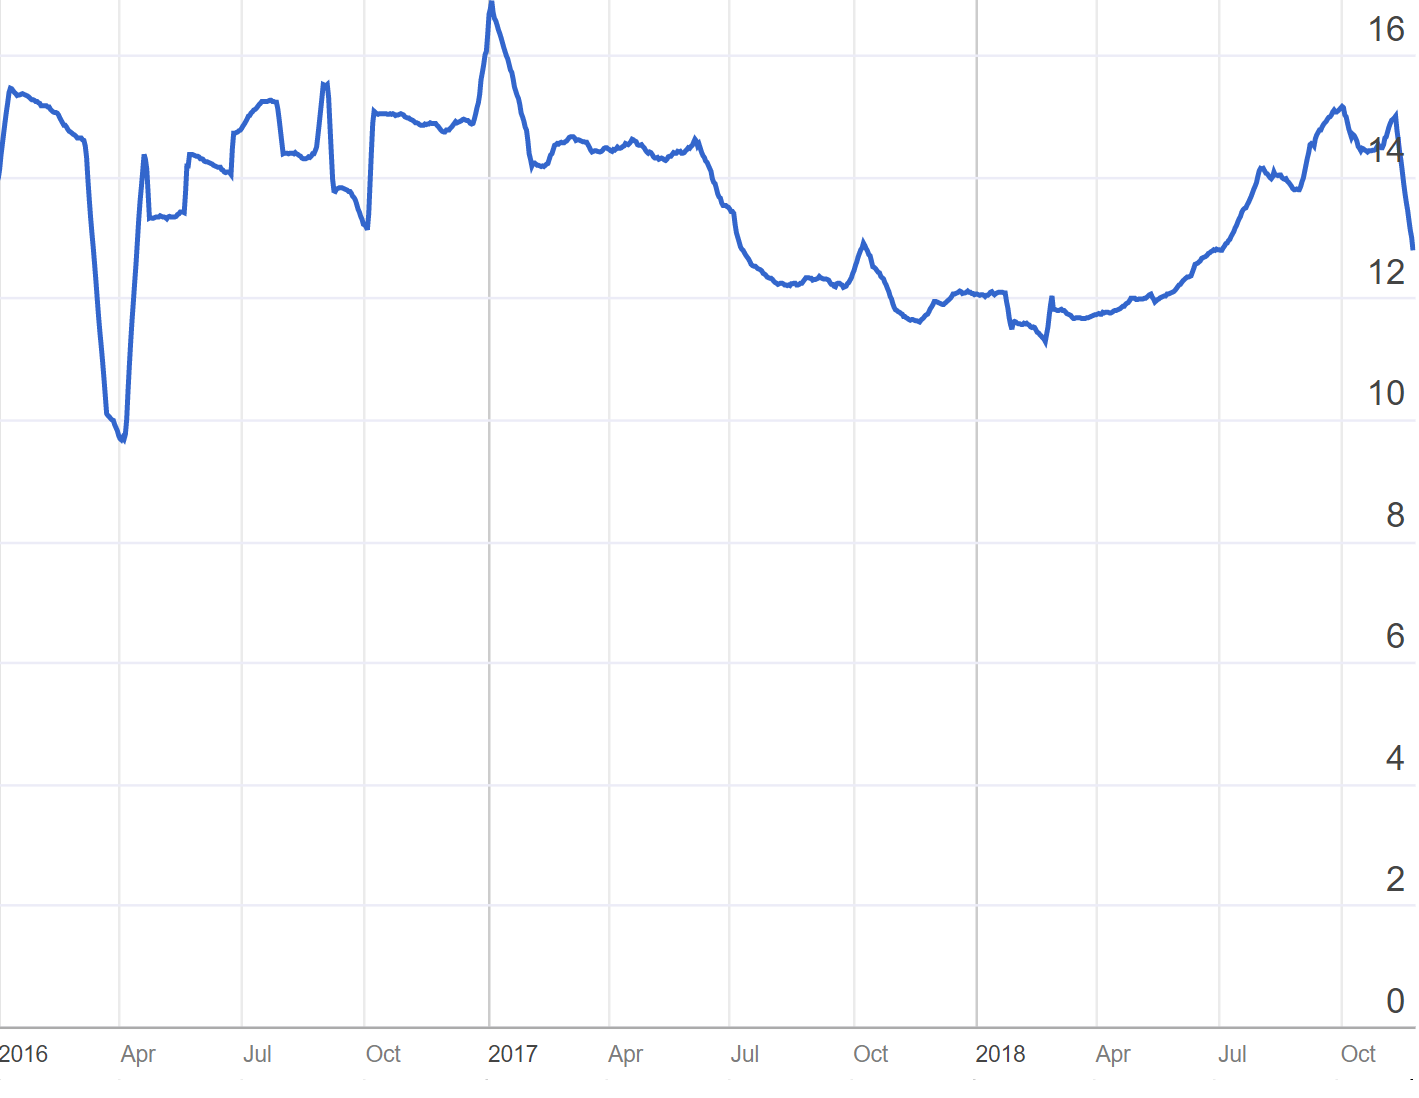
\includegraphics[width=0.95\linewidth]{apnic.png}
    \caption{APNIC estimate of global DNS resolvers (Google PDNS as well as
    local resolvers) performing DNSSEC validation from January 2016 to December
    2018.}\label{fig:apnic}
\end{figure}

It should be noted that DNSSEC does not necessarily make the DNS network---\ie{}
properly configured DNS servers---more vulnerable to amplification or other types
of reflection attacks~\cite{Ariya} than it already is as a UDP-based content
delivery service~\cite{USCERT, Vixie}.

\TODO{This section sounds super negative.  Maybe end by noting that
  DNSSEC is just one way to support the backend of this idea and that
  even if DNSSEC isn't adopted, then the key idea is still valid and
  can be implemented by storing the authoritative hash in a DHT (or
  maybe something else as well)?}

\subsubsection{DNS-Specific Protocol Limitations}

DNS~\cite{DNS1} was not originally designed to transport or store relatively
large amounts of data, though this has been addressed with EDNS0~\cite{EDNS}.
The checksums stored in DNS should not be much longer than 128 bytes or the
output of the SHA512 function. Regardless, DNS resource record extensions exist
that store much more than 128 bytes of data~\cite{CERT, IPSECKEY, DANE3, DANE1}.

Several working groups are considering DNS as a storage medium for
checksums/hash output as well, such as securitytxt~\cite{draft-sectxt}. A widely
deployed example of DNS ``TXT'' resource records being used this way is SPF and
DKIM~\cite{DKIM}.

Additionally, \SYSTEM{} does not add to the danger of amplification and other
reflection attacks on DNS; these are generic DNS issues addressable at other
layers of the protocol.

\TODO{In contrast to the previous section, this one doesn't seem like
  limitations at all.  Not sure anything needs to change here, but it
  is a striking contrast.

\subsubsection{Chrome Implementation}

Our current JavaScript proof-of-concept implementation, as a Chrome extension,
is not allowed to touch the resource file downloaded by Chrome and so cannot
prevent the potentially-malicious resource file from being executed by the end
user---a feature Chrome/Chromium reserves for its own internal use. The Chrome
\textit{app} API~\cite{AppAPI} might have been of assistance as it allowed for
some limited filesystem traversal via a now deprecated native app API; there is
also a non-standard HTML5/WebExtensions FileSystem API that would provide
similar functionality were it to be widely considered~\cite{deadSpec}.

\SYSTEM{} would be even more effective as a browser extension if Chrome/Chromium
or the WebExtensions API allowed for an explicit \texttt{onComplete} event hook
in the downloads API. This hook would fire immediately before a file download
completed and the file became executable, \ie had its \texttt{.crdownload} or
\texttt{.download} extension removed. The hook would consume a
\texttt{Promise}/\texttt{AsyncFunction} that kept the download in its
non-complete state until said \texttt{Promise} completed. This would allow
\SYSTEM{}'s background page to do something like alter the download's
\texttt{DangerType} property and alert the end user to the dangerous download
naturally. This would have the advantage of communicating intent through the
browser's familiar UI and preventing the potentially-malicious download from
becoming immediately executable. Unfortunately, the closest the
Chrome/WebExtensions API comes to allowing \texttt{DangerType} mutations is the
\texttt{acceptDanger} method on the downloads API, but it is not suitable for
use with \SYSTEM{} as a background page based extension.

\subsection{Future Work}

\subsubsection{Merkle Trees and Early Resource Validation}

Using Merkle Trees instead of pure hashing functions would enable partial
verification of large files; \ie{} if the file we are downloading is 10TiB, we
do not have to wait for it to finish downloading before we render a failing
judgement. This saves the user time. Perhaps using the Tiger hash, since Tiger
Merkle Trees seem to be popular among large P2P and file sharing applications.
\TODO{LAst sentence is incomplete}.

\subsubsection{Replacing RIs with URNs}

The goal of the Resource Identifiers (RI) is very similar to that of Uniform
Resource Names (URN). It may make sense to replace the mapping between RIs and
Authoritative Hashes with purely URN-based DNS lookups that return specially
formatted TXT records upon success. This would further simplify the deployment
process for service administrators since DNS updates would be based upon the
resource's contents instead of both its contents \textit{and where it is located
physically on a distribution server}. It may also allow for additional
confirmation methods of the identical resources in different domains and in
different locations.

We did not choose a URN-based scheme in our initial approach due to a new URN
scheme requiring the registration of a unique identifier with the Internet
Assigned Numbers Authority. Going forward, we can potentially adopt a URN scheme
that already exists, such as Magnet links~\cite{MagnetLinks} or the informal
IETF draft for hash-based URN namespaces~\cite{draft-URN}. With URNs, we can
ensure our naming scheme is based solely on a resource's contents rather than
both its contents and its location on a web server.

\section{Conclusion} \label{sec:conclusion}

Downloading resources over the internet is indeed a risky endeavor. Resource
integrity attacks, and Supply Chain Attacks more broadly, are becoming more
frequent and their impact more widely felt. This paper shows that the de facto
standard for addressing resource integrity risk---the use of \emph{checksums}
coupled with a secure transport layer---is an insufficient and often ineffective
solution. We propose a novel resource validation scheme meant as a complete
replacement for checksum based approaches: \SYSTEM{}, which automates the
tedious parts of verification to eliminate user apathy while leveraging
highly-available authenticated distributed systems to ensure resources and
checksums are not co-hosted. Further, we demonstrate the effectiveness and
practicality of our approach versus resource integrity attacks in real-world
systems.

The results of our evaluation show that \SYSTEM{} is more effective than
checksums and other existing solutions at mitigating resource integrity attacks
against arbitrary resources on the internet. Further, we show \SYSTEM{} detects
a wide variety of real-world integrity errors across a diverse set of platforms.
\SYSTEM{} is both scalable and immediately deployable for organizations that
secure their DNS zone(s) with DNSSEC.

We make our DNS implementation of \SYSTEM{} available open source so that others
can extend it or compare to it. Our hope is that this work motivates further
exploration of resource integrity Supply Chain Attack mitigation
methods.~\footnote{The \SYSTEM{} Chrome extension is available at
https://tinyurl.com/dnschk-actual}.


\clearpage
\printbibliography
\end{document}
